\chapter{Uvod}
Diplomska naloga je ponovna implementacija in nadgradnja interaktivne
umetniške instalacije ``15 sekund slave''~\cite{15secLeonardo}. Motivacija za
instalacijo je umetniško delovanje ameriškega pop-art umetnika Andyja Warhola.
``15 sekund slave'' izgleda kot klasična slika, a je dejansko računalniški
zaslon, okvirjen kot umetniška slika. Nad zaslonom je v okviru vgrajen
digitalni fotoaparat, ki je povezan z računalnikom v ozadju. Vsakih 15 sekund
fotoaparat slika obiskovalce galerije, ki stojijo pred sliko. Na sliki
računalniški program poišče vse obraze in nato naključno izbere enega izmed
njih. Ta obraz nato z grafičnimi filtri program obdela tako, da pridobi tako
imenovani ``pop-art'' videz z manjšim številom živih barv, ki spominjajo na
slike slavnih osebnosti, ki jih je iz fotografij delal Andy Warhol. Ker je
prvotna instalacija nastala pred več kot 10 leti in se je strojna oprema v tem
času že zelo spremenila, se je pokazala potreba po prilagoditvi aplikacije
novemu stanju tehnologije \cite{trifonova}.

V magistrski nalogi najprej preučite splošne probleme pri vzdrževanju
umetniških instalacij, ki temeljijo na računalniški tehnologiji
\cite{miller1,miller2,digitalartconservation}. Zaradi hitrega napredka
računalniške tehnologije je potrebno take aplikacije po eni strani prilagajati
novi strojni in sistemski programski opremi, pa tudi novim funkcionalnim
možnostim, ki jih nove tehnologije nudijo. Po drugi strani, pa z umetniškega
vidika običajno želimo, da se zunanja pojava umetniškega dela ne spremeni. V
konkretnem primeru instalacije ``15 sekund slave'' namesto računalnika in
digitalnega fotoaparata uporabite mobilni telefon z vgrajeno kamero ter
možnostjo brezžičnega prenosa podatkov. V enem načinu delovanja nove
implementacije instalacije, se naj zunanji izgled, način uporabe in generirane
slike ne razlikujejo od prvotne instalacije. V drugem načinu delovanja nove
implementacije pa poiščite nove, kreativne načine funkcioniranja, ki jih
omogoča novejša tehnologija. Tu je mišljena predvsem uporaba videa namesto
statične slike in povezovanje s socialnimi omrežji.


\chapter{Obdelava slik}
Instalacija ``15 sekund slave'' vsebuje 17 različnih
filtrov~\cite[Poglavje~5]{diplomskaSamoJuvan} za obdelavo prejetih slik v pop-
art slike. Filtri so bili izdelani s pomočjo grafičnega programa GIMP.


\section{GIMP}
GIMP je odprto-kodno programsko orodje za obdelavo slik.


\subsection{Zgodovina}
Začetek projekta sega v leto 1995, kot semestrski projekt v Univerzi
Kalifornije, Berkeley. Kot prva avtorja, Spencer Kimball in Peter Mattis sta
projekt poimenovala \textit{angl. General Image Manipulation Program}. Malo
kasneje, ko je univerzo obiskal Richard Stallman sta ga prosila, če lahko
zamenjata besedo ``General'' v ``GNU''. Od takrat naprej se program imenuje
\textit{angl. GNU Image Manipulation Program} ali na kratko še vedno
GIMP~\cite{wiki:GIMP}.


\section{Izbira filtrov}
Že prvotna izbira filtrov je izhajala iz programskega orodja za predelavo slik
GIMP. Zaradi lažjega dela se je najprej grafičnega vmesnika izbralo zaporedje
različnih filtrov z različnimi parametri. Izbrani so bili naslednji filtri:
\begin{itemize}
    \item \textbf{uravnovešanje barv v RGB prostoru} \textit{angl. color balance} \hfill \\
        Prekrije celotno sliko z barvo v izbranem odtenku.
    \item \textbf{posteriziranje} \textit{angl. posterize} \hfill \\
        Zmanjšuje število barv na sliki.
    \item \textbf{uravnovešanje barv v HSL prostoru} \textit{angl. hue saturation balance} \hfill \\
        Spreminja odtenke barv, svetlost in intenzivnost na sliki.
\end{itemize}


\section{Implementacija filtrov}
Ker je GIMP odprto-koden smo imeli tudi dostop do implementacije filtrov.
Implementacije filtrov so napisani v programskem jeziku C. Na prvi pogled kot
nalašč za enostaven prenos na Android platformo preko JNI. Vendar pa so se
pokazale težave, saj so bili filtri močno povezani z GIMP objekti ter nekoliko
bolj kompleksni, kot smo mi potrebovali. Zato smo se odločili, da vzamemo samo
algoritem oziroma idejo za tem, ter implementiramo po naših potrebah. Naredili
smo tri različne implementacije in jih med seboj primerjali.

Prva implementacija je napisana v programskem jeziku java. Izkazalo se je kot
zelo počasno. Orodje za sproščanje pomnilnika GC \textit{(angl. garbage
collector)} se je klical velikokrat, kar je posledično porabilo več kot nekaj
sekund za filter. Tega si nismo mogli privoščiti, zato smo iskali alternative.

Naslednja implementacija je napisana s pomočjo grafične kartice in sicer z
orodjem OPENGL ES, verzije 2.0. Čas porabe pri izvajanju se je občutno
zmanjšal. Ko so bile teksture zapisane na grafični kartici so se filtri
izvajali v manj kot sekundi. Ta rešitev je bila že dovolj dobra, vendar pa se
nam je zdelo, da je uporaba grafične kartice za tako lahke operacije potrata
energije.

Čeprav so bili rezultati že dovolj dobri, smo se odločili še za implementacijo
v programskem jeziku C. Rezultati so pokazali, da je ta rešitev malo bolj
počasna kot prejšnja, vendar pa za to nismo potrebovali grafične kartice na
telefonu. Čas porabe je bil manj kot sekundo za filter.

\subsection{HSL barvni prostor}
\label{sec:hsl}

\begin{align}
R, G, B &\in [0,255] \nonumber \\
Cmax &= max(R, G, B) \\
Cmin &= min(R, G, B) \\
\Delta &= (Cmax - Cmin)
\end{align}

\begin{equation}
L = (max + min) / 2 \label{eq:hsl_l}
\end{equation}

\begin{equation}
S =
\begin{cases}
    0 \text{,}& \Delta = 0 \\
    255 * \Delta / (Cmax + Cmin) \text{,}& L < 128 \\
    255 * \Delta / (511 - Cmax - Cmin) \text{,}& \text{ostalo}
\end{cases}
\end{equation}

\begin{equation}
H' =
\begin{cases}
    0 \text{,}& \Delta = 0 \\
    0 + 42.5 * (G - B) / \Delta \text{,}& R = Cmax \\
    85 + 42.5 * (B - R) / \Delta \text{,}& G = Cmax \\
    170 + 42.5 * (R - G) / \Delta \text{,}& B = Cmax
\end{cases}
\end{equation}

\begin{equation}
H =
\begin{cases}
    H' + 255 \text{,}& H' < 0 \\
    H' - 255 \text{,}& H' > 255 \\
    H' \text{,}& \text{ostalo}
\end{cases}
\end{equation}

\begin{lstlisting}[caption=algoritem]
Cmax = max(R, G, B)

\end{lstlisting}

\subsection{uravnovešanje barv v RGB prostoru}

\begin{equation}
clamp_{min}^{max}(x) =
\begin{cases}
    min \text{,}& x < min \\
    max \text{,}& x > max \\
    x \text{,}& \text{ostalo}
\end{cases}
\end{equation}

\begin{align}
shadows(x) &= clamp_{0}^{1}(\frac{117 - x}{64}) * 1.785 \\
color\_balance(x, x') &= clamp_{0}^{255}(x + x' * shadows(x)) \label{eq:color_balance}
\end{align}

Uravnovešanje barv se računa v barvnem prostoru RGB. Računamo jo za vsako
barvo posebej, in sicer z enačbo~\eqref{eq:color_balance}, kjer je $x$ enak
originalni barvi, $x'$ pa barvi, s katero želimo uravnovesiti originalno barvo
$x$. $x$ in $x'$ sta pozitivni celi števili med 0 in 255.

Po izračunanih vrednosti dane rezultate v RGB prostoru prenesemo v HSL prostor
s pomočjo enačb, napisnih v poglavju~\ref{sec:hsl}. Tako dobimo $H$, $S$ in
$L$. Iz originalnih vrednosti, to je vrednost barve na sliki, izračunamo
$L$~\ref{eq:hsl_l} in ga nadomestimo s prejšnjim, zato da ohranimo podobno
svetlost. $H$, $S$ in novo pridobljeni $L$ spremenimo nazaj v RGB prostor.

\subsection{Posteriziranje}

\begin{equation}
luts(x, levels) = 255 * \frac{\left \lfloor{\frac{x}{255} * (levels - 1) + 0.5}\right \rfloor}{levels - 1} + 0.5
\end{equation}

Posteriziranje se računa v barvnem prostoru RGB...

\subsection{Uravnovešanje barv v HSL prostoru}

\begin{align}
htv(x, x') &= x + 255 * \frac{x'}{360} \nonumber \\
hue\_transfer(x, x') &=
\begin{cases}
    htv(x, x') + 255 \text{,}& htv(x, x') < 0 \\
    htv(x, x') - 255 \text{,}& htv(x, x') > 255 \\
    htv(x, x') \text{,}& \text{ostalo}
\end{cases}
\end{align}

\begin{align}
ltv(x, x') &= clamp_{-255}^{255}(1.27 * x') \nonumber \\
lightness\_transfer(x, x') &=
\begin{cases}
    x * \frac{255 + ltv(x, x')}{255} \text{,}& ltv(x, x') < 0 \\
    x + \frac{(255 - x) * ltv(x, x')}{255} \text{,}& ltv(x, x') \geq 0
\end{cases}
\end{align}

\begin{align}
stv(x, x') &= clamp_{-255}^{255}(2.25 * x') \nonumber \\
saturation\_transfer(x, x') &= clamp_{0}^{255}(x + x * \frac{stv(x, x')}{255})
\end{align}

\subsubsection*{Filter 1}
Prvi filter je sestavljen iz dveh osnovnih filtrov. Najprej sliko obdelamo s
filtrom ``uravnovešanje barv'' in sicer s parametri $R = 30$, $G = -32$ in
$B = 16$. Rezultat obdelamo še s filtrom ``posteriziranje'' s parametrom
$ST =4$. Rezultat testne slike lahko vidimo na sliki~\ref{fig:lena_filter_1}.

\begin{figure}[h]
    \centering
    \begin{subfigure}[b]{0.4\textwidth}
        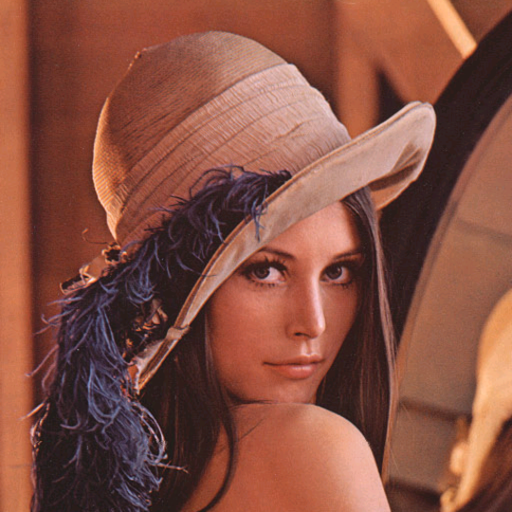
\includegraphics[width=\textwidth]{lena}
        \caption{Original}
    \end{subfigure}
    \begin{subfigure}[b]{0.4\textwidth}
        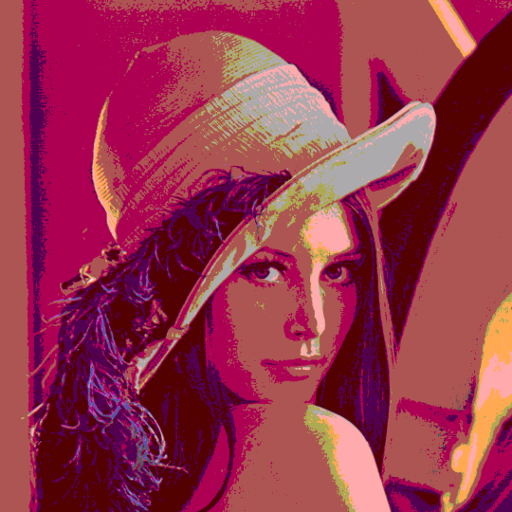
\includegraphics[width=\textwidth]{lena_filter_1}
        \caption{Prvi filter}
    \end{subfigure}
    \caption{Primerjava originalne slike z obdelano sliko}
    \label{fig:lena_filter_1}
\end{figure}


\subsubsection*{Filter 2}
Drugi filter je sestavljen iz dveh osnovnih filtrov. Najprej sliko obdelamo s
filtrom ``uravnovešanje barv'' in sicer s parametri $R = -36$, $G = -37$ in
$B = 39$. Rezultat obdelamo še s filtrom ``posteriziranje'' s parametrom
$ST = 4$. Rezultat testne slike lahko vidimo na sliki~\ref{fig:lena_filter_2}.

\begin{figure}[h]
    \centering
    \begin{subfigure}[b]{0.4\textwidth}
        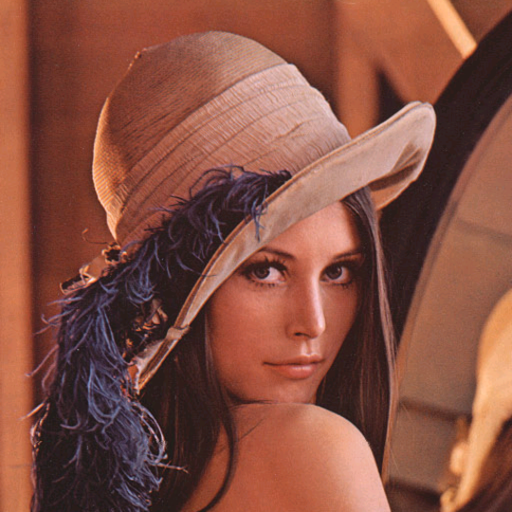
\includegraphics[width=\textwidth]{lena}
        \caption{Original}
    \end{subfigure}
    \begin{subfigure}[b]{0.4\textwidth}
        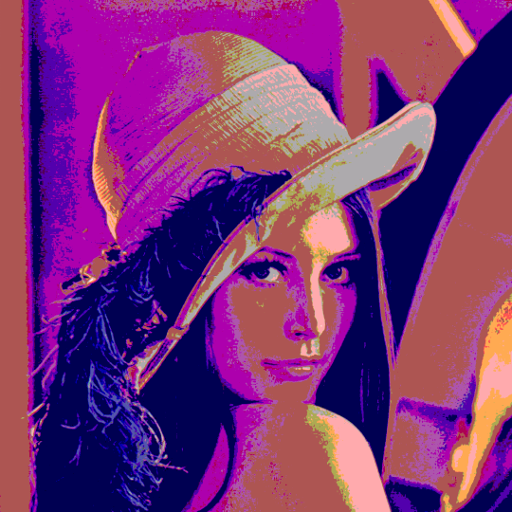
\includegraphics[width=\textwidth]{lena_filter_2}
        \caption{Drugi filter}
    \end{subfigure}
    \caption{Primerjava originalne slike z obdelano sliko}
    \label{fig:lena_filter_2}
\end{figure}


\subsubsection*{Filter 3}
Tretji filter vsebuje le osnovni filter ``posteriziranje'' in sicer s parametrom
$ST = 2$. Rezultat testne slike lahko vidimo na sliki~\ref{fig:lena_filter_3}.

\begin{figure}[h]
    \centering
    \begin{subfigure}[b]{0.4\textwidth}
        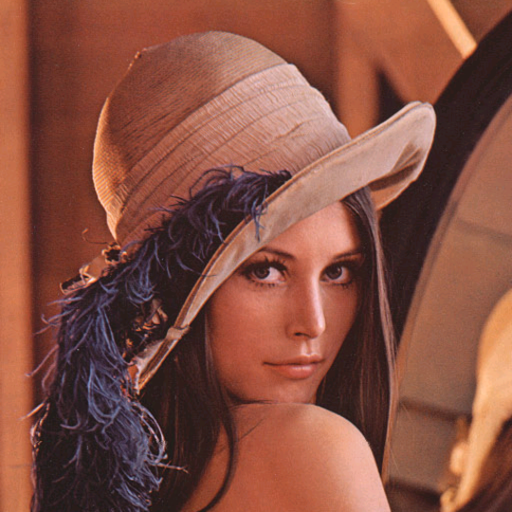
\includegraphics[width=\textwidth]{lena}
        \caption{Original}
    \end{subfigure}
    \begin{subfigure}[b]{0.4\textwidth}
        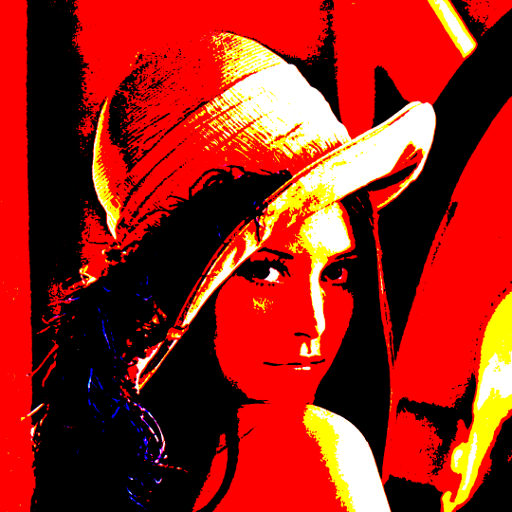
\includegraphics[width=\textwidth]{lena_filter_3}
        \caption{Tretji filter}
    \end{subfigure}
    \caption{Primerjava originalne slike z obdelano sliko}
    \label{fig:lena_filter_3}
\end{figure}


\subsubsection*{Filter 4}
Četrti filter je sestavljen iz dveh osnovnih filtrov. Najprej sliko obdelamo s
filtrom ``uravnovešanje barv'' in sicer s parametri $R = 100$, $G = -100$ in
$B = -100$. Rezultat obdelamo še s filtrom ``posteriziranje'' s parametrom
$ST = 3$. Rezultat testne slike lahko vidimo na sliki~\ref{fig:lena_filter_4}.

\begin{figure}[h]
    \centering
    \begin{subfigure}[b]{0.4\textwidth}
        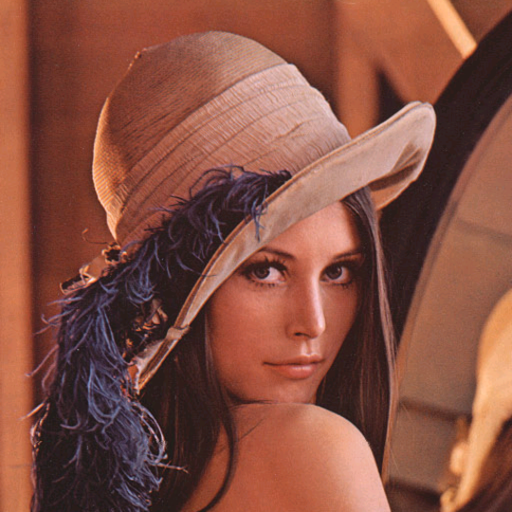
\includegraphics[width=\textwidth]{lena}
        \caption{Original}
    \end{subfigure}
    \begin{subfigure}[b]{0.4\textwidth}
        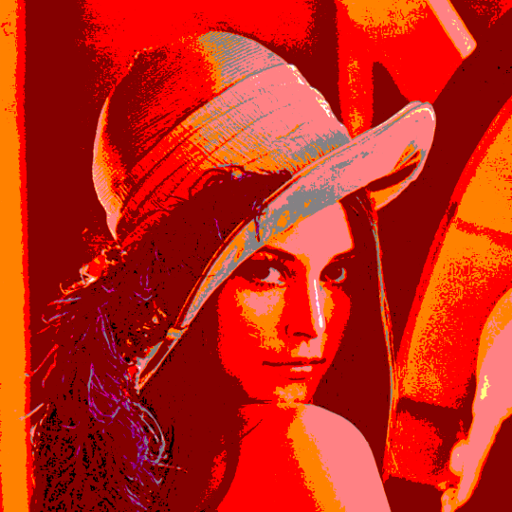
\includegraphics[width=\textwidth]{lena_filter_4}
        \caption{Četrti filter}
    \end{subfigure}
    \caption{Primerjava originalne slike z obdelano sliko}
    \label{fig:lena_filter_4}
\end{figure}


\subsubsection*{Filter 5}
Peti filter je sestavljen iz dveh osnovnih filtrov. Najprej sliko obdelamo s
filtrom ``uravnovešanje barv'' in sicer s parametri $R = -100$, $G = -100$ in
$B = 100$. Rezultat obdelamo še s filtrom ``posteriziranje'' s parametrom
$ST = 3$. Rezultat testne slike lahko vidimo na sliki~\ref{fig:lena_filter_5}.

\begin{figure}[h]
    \centering
    \begin{subfigure}[b]{0.4\textwidth}
        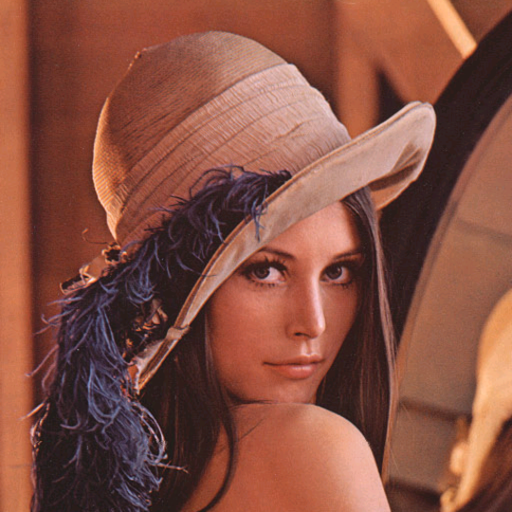
\includegraphics[width=\textwidth]{lena}
        \caption{Original}
    \end{subfigure}
    \begin{subfigure}[b]{0.4\textwidth}
        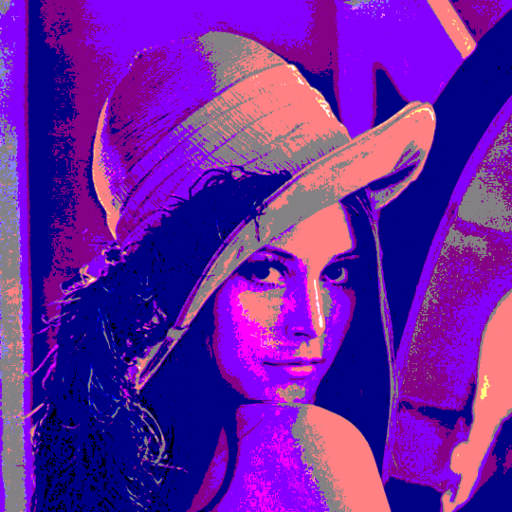
\includegraphics[width=\textwidth]{lena_filter_5}
        \caption{Peti filter}
    \end{subfigure}
    \caption{Primerjava originalne slike z obdelano sliko}
    \label{fig:lena_filter_5}
\end{figure}


\subsubsection*{Filter 6}
Šesti filter je sestavljen iz dveh osnovnih filtrov. Najprej sliko obdelamo s
filtrom ``uravnovešanje barv'' in sicer s parametri $R = -100$, $G = 100$ in
$B = -100$. Rezultat obdelamo še s filtrom ``posteriziranje'' s parametrom
$ST = 3$. Rezultat testne slike lahko vidimo na sliki~\ref{fig:lena_filter_6}.

\begin{figure}[h]
    \centering
    \begin{subfigure}[b]{0.4\textwidth}
        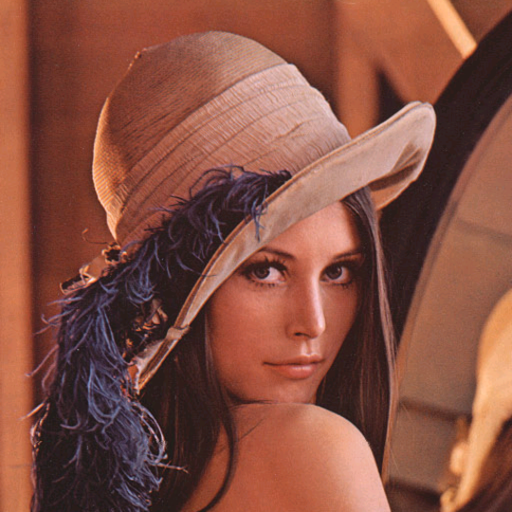
\includegraphics[width=\textwidth]{lena}
        \caption{Original}
    \end{subfigure}
    \begin{subfigure}[b]{0.4\textwidth}
        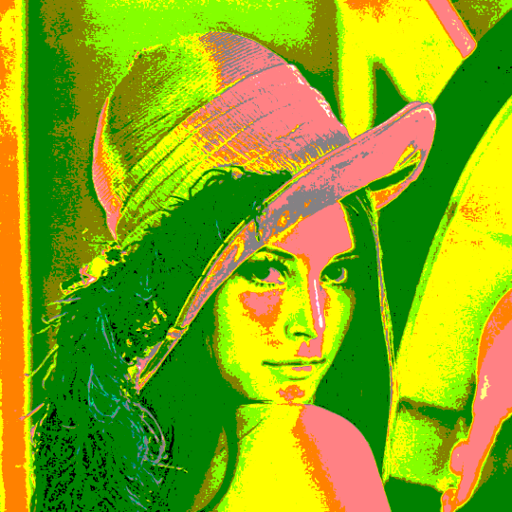
\includegraphics[width=\textwidth]{lena_filter_6}
        \caption{Šesti filter}
    \end{subfigure}
    \caption{Primerjava originalne slike z obdelano sliko}
    \label{fig:lena_filter_6}
\end{figure}


\subsubsection*{Filter 7}
Sedmi filter je sestavljen iz dveh osnovnih filtrov. Najprej sliko obdelamo s
filtrom ``posteriziranje'' in sicer s parametrom $ST = 5$. Rezultat obdelamo
še s filtrom ``uravnovešanje barv v HSL prostoru'' s parametri $H = -41$,
$L = -15$ in $S = 6$. Rezultat testne slike lahko vidimo na
sliki~\ref{fig:lena_filter_7}.

\begin{figure}[h]
    \centering
    \begin{subfigure}[b]{0.4\textwidth}
        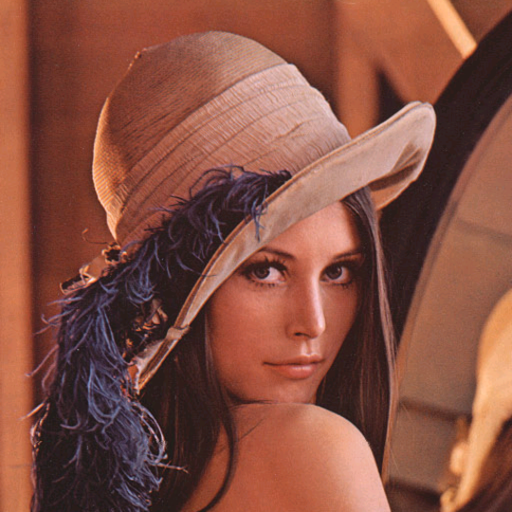
\includegraphics[width=\textwidth]{lena}
        \caption{Original}
    \end{subfigure}
    \begin{subfigure}[b]{0.4\textwidth}
        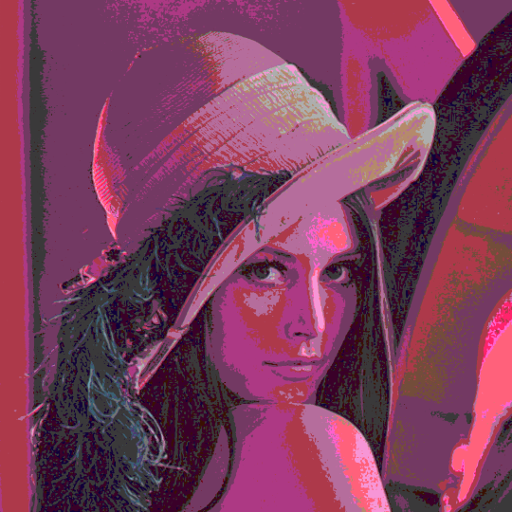
\includegraphics[width=\textwidth]{lena_filter_7}
        \caption{Sedmi filter}
    \end{subfigure}
    \caption{Primerjava originalne slike z obdelano sliko}
    \label{fig:lena_filter_7}
\end{figure}


\subsubsection*{Filter 8}
Osmi filter je sestavljen iz dveh osnovnih filtrov. Najprej sliko obdelamo s
filtrom ``posteriziranje'' in sicer s parametrom $ST = 6$. Rezultat obdelamo
še s filtrom ``uravnovešanje barv'' s parametri $R = -29$, $G = 40$ in $B = 100$.
Rezultat testne slike lahko vidimo na sliki~\ref{fig:lena_filter_8}.

\begin{figure}[h]
    \centering
    \begin{subfigure}[b]{0.4\textwidth}
        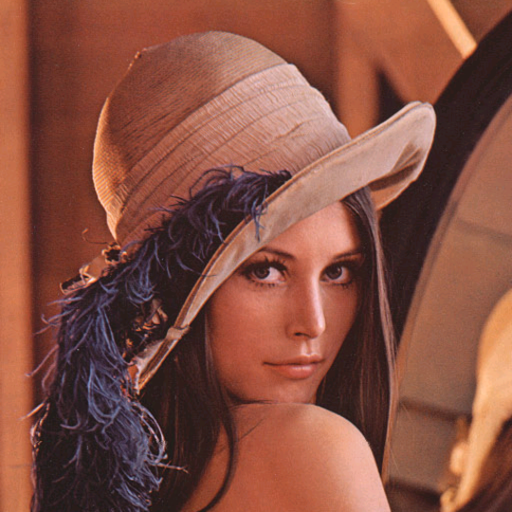
\includegraphics[width=\textwidth]{lena}
        \caption{Original}
    \end{subfigure}
    \begin{subfigure}[b]{0.4\textwidth}
        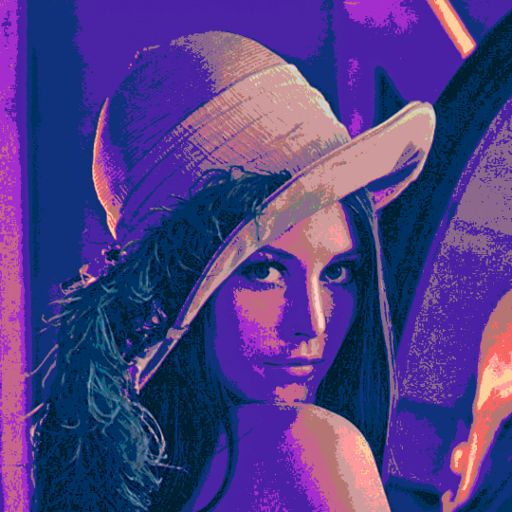
\includegraphics[width=\textwidth]{lena_filter_8}
        \caption{Osmi filter}
    \end{subfigure}
    \caption{Primerjava originalne slike z obdelano sliko}
    \label{fig:lena_filter_8}
\end{figure}


\subsubsection*{Filter 9}
Deveti filter je sestavljen iz dveh osnovnih filtrov. Najprej sliko obdelamo s
filtrom ``uravnovešanje barv v HSL prostoru'' in sicer s parametri $H = -41$,
$L = -20$ in $S = 25$. Rezultat obdelamo še s filtrom ``posteriziranje'' s
parametrom $ST = 4$. Rezultat testne slike lahko vidimo na
sliki~\ref{fig:lena_filter_9}.

\begin{figure}[h]
    \centering
    \begin{subfigure}[b]{0.4\textwidth}
        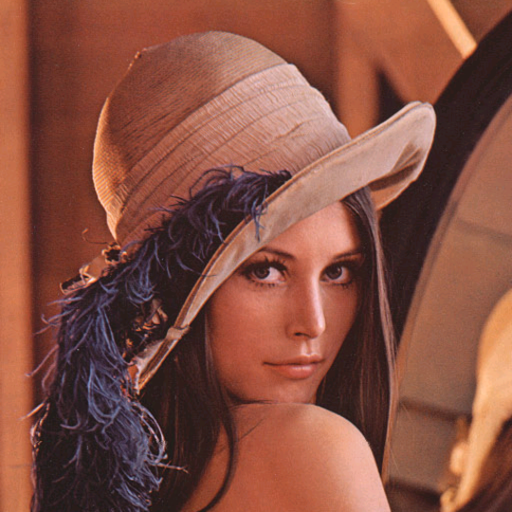
\includegraphics[width=\textwidth]{lena}
        \caption{Original}
    \end{subfigure}
    \begin{subfigure}[b]{0.4\textwidth}
        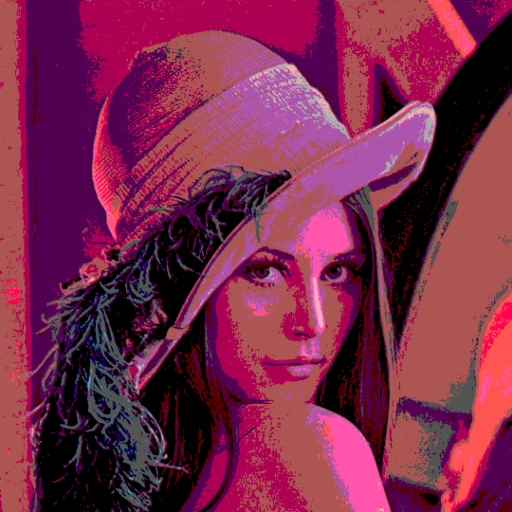
\includegraphics[width=\textwidth]{lena_filter_9}
        \caption{Deveti filter}
    \end{subfigure}
    \caption{Primerjava originalne slike z obdelano sliko}
    \label{fig:lena_filter_9}
\end{figure}


\subsubsection*{Filter 10}
Deseti filter je sestavljen iz treh osnovnih filtrov. Najprej sliko obdelamo s
filtrom ``uravnovešanje barv'' in sicer s parametri $R = 100$, $G = -100$ in
$B = -100$. Rezultat obdelamo še s filtrom ``posteriziranje'' s parametrom
$ST= 3$ in nazadnje še s filtrom ``uravnovešanje barv v HSL prostoru'' s
parametri $H = -41$, $L = -10$ in $S = 20$. Rezultat testne slike lahko
vidimo na sliki~\ref{fig:lena_filter_10}.

\begin{figure}[h]
    \centering
    \begin{subfigure}[b]{0.4\textwidth}
        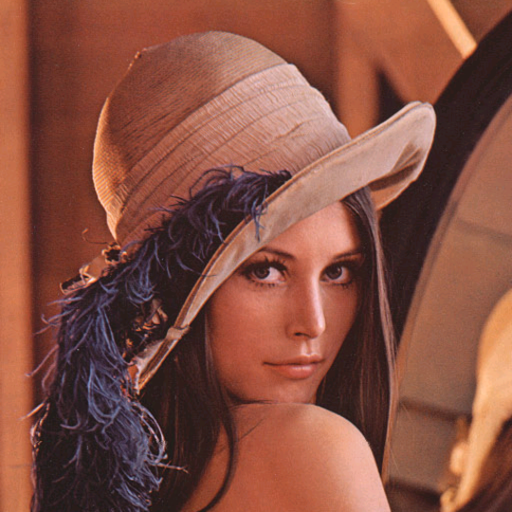
\includegraphics[width=\textwidth]{lena}
        \caption{Original}
    \end{subfigure}
    \begin{subfigure}[b]{0.4\textwidth}
        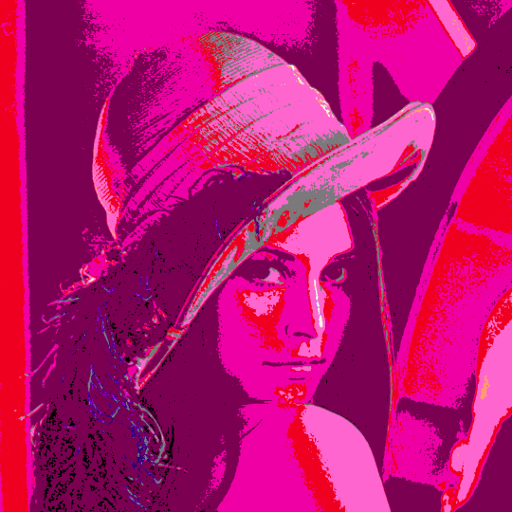
\includegraphics[width=\textwidth]{lena_filter_10}
        \caption{Deseti filter}
    \end{subfigure}
    \caption{Primerjava originalne slike z obdelano sliko}
    \label{fig:lena_filter_10}
\end{figure}


\subsubsection*{Filter 11}
Enajsti filter je sestavljen iz treh osnovnih filtrov. Najprej sliko obdelamo s
filtrom ``uravnovešanje barv'' in sicer s parametri $R = 34$, $G = -38$ in
$B = 24$. Rezultat obdelamo še s filtrom ``posteriziranje'' s parametrom
$ST= 4$ in nazadnje še s filtrom ``uravnovešanje barv v HSL prostoru'' s
parametri $H = -65$, $L = 0$ in $S = 0$. Rezultat testne slike lahko
vidimo na sliki~\ref{fig:lena_filter_11}.

\begin{figure}[h]
    \centering
    \begin{subfigure}[b]{0.4\textwidth}
        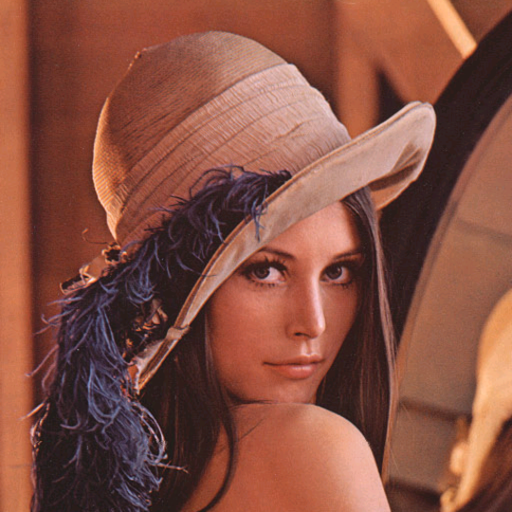
\includegraphics[width=\textwidth]{lena}
        \caption{Original}
    \end{subfigure}
    \begin{subfigure}[b]{0.4\textwidth}
        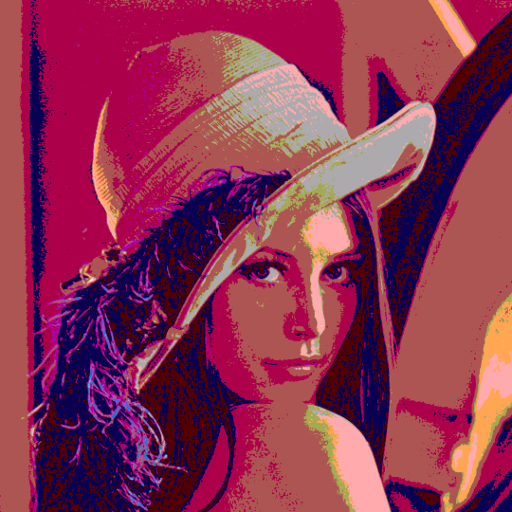
\includegraphics[width=\textwidth]{lena_filter_11}
        \caption{Enajsti filter}
    \end{subfigure}
    \caption{Primerjava originalne slike z obdelano sliko}
    \label{fig:lena_filter_11}
\end{figure}


\subsubsection*{Filter 12}
Dvanajsti filter je sestavljen iz dveh osnovnih filtrov. Najprej sliko obdelamo s
filtrom ``uravnovešanje barv'' in sicer s parametri $R = 40$, $G = -40$ in
$B = 28$. Rezultat obdelamo še s filtrom ``posteriziranje'' s parametrom
$ST= 4$ in nazadnje še enkrat s filtrom ``uravnovešanje barv'' vendar s
parametri $R = -100$, $G = -42$ in $B = 100$. Rezultat testne slike lahko
vidimo na sliki~\ref{fig:lena_filter_12}.

\begin{figure}[h]
    \centering
    \begin{subfigure}[b]{0.4\textwidth}
        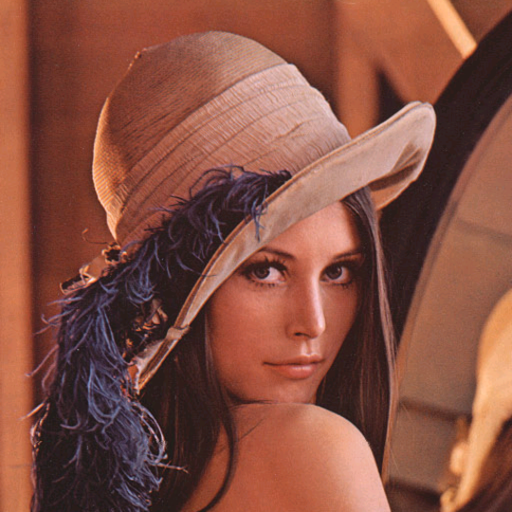
\includegraphics[width=\textwidth]{lena}
        \caption{Original}
    \end{subfigure}
    \begin{subfigure}[b]{0.4\textwidth}
        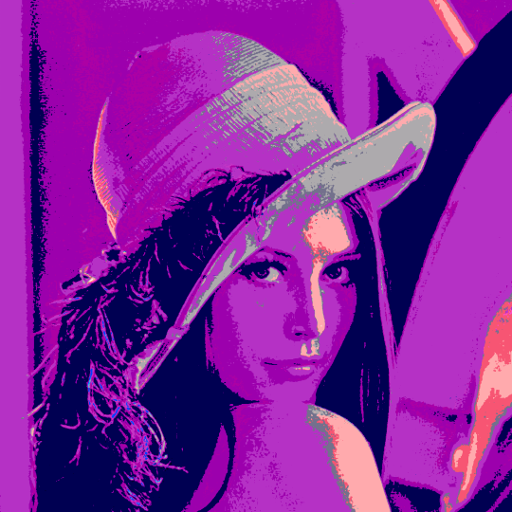
\includegraphics[width=\textwidth]{lena_filter_12}
        \caption{Dvanajsti filter}
    \end{subfigure}
    \caption{Primerjava originalne slike z obdelano sliko}
    \label{fig:lena_filter_12}
\end{figure}


\subsubsection*{Filter 13}
\begin{figure}[h]
    \centering
    \begin{subfigure}[b]{0.4\textwidth}
        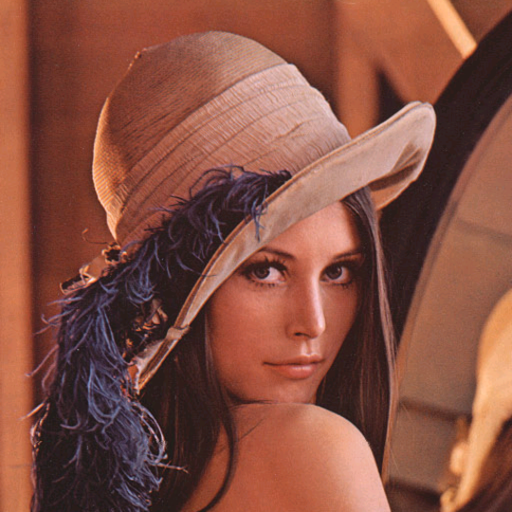
\includegraphics[width=\textwidth]{lena}
        \caption{Original}
    \end{subfigure}
    \begin{subfigure}[b]{0.4\textwidth}
        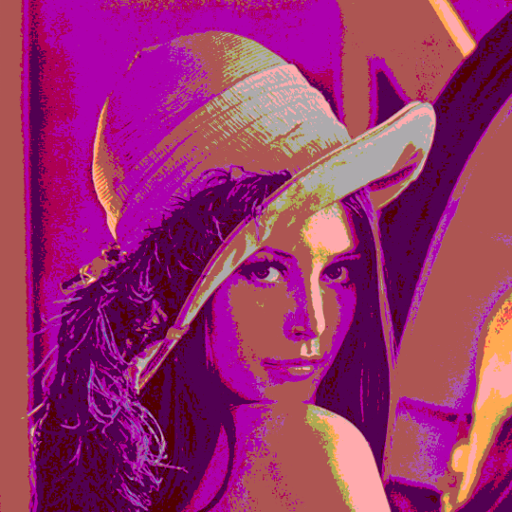
\includegraphics[width=\textwidth]{lena_filter_13}
        \caption{Trinajsti filter}
    \end{subfigure}
    \caption{Primerjava originalne slike z obdelano sliko}
    \label{fig:lena_filter_13}
\end{figure}


\subsubsection*{Filter 14}
\begin{figure}[h]
    \centering
    \begin{subfigure}[b]{0.4\textwidth}
        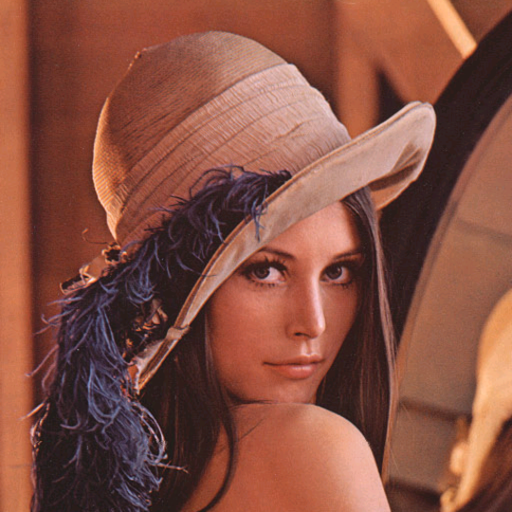
\includegraphics[width=\textwidth]{lena}
        \caption{Original}
    \end{subfigure}
    \begin{subfigure}[b]{0.4\textwidth}
        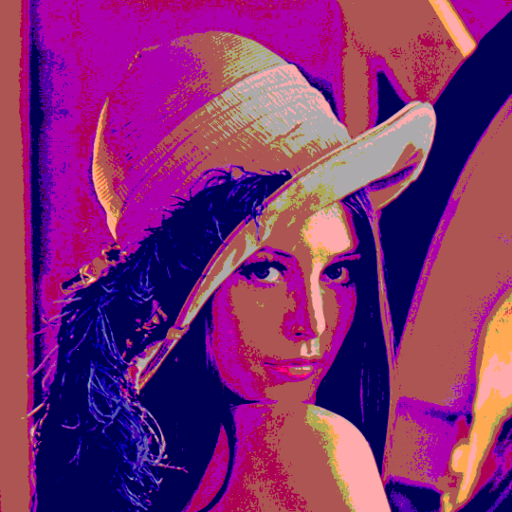
\includegraphics[width=\textwidth]{lena_filter_14}
        \caption{Štirinajsti filter}
    \end{subfigure}
    \caption{Primerjava originalne slike z obdelano sliko}
    \label{fig:lena_filter_14}
\end{figure}


\subsubsection*{Filter 15}
\begin{figure}[h]
    \centering
    \begin{subfigure}[b]{0.4\textwidth}
        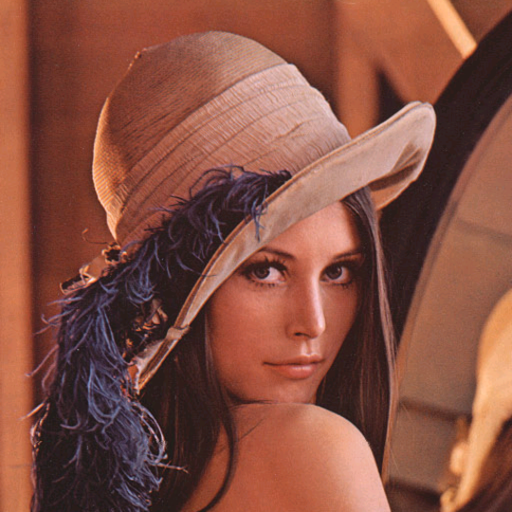
\includegraphics[width=\textwidth]{lena}
        \caption{Original}
    \end{subfigure}
    \begin{subfigure}[b]{0.4\textwidth}
        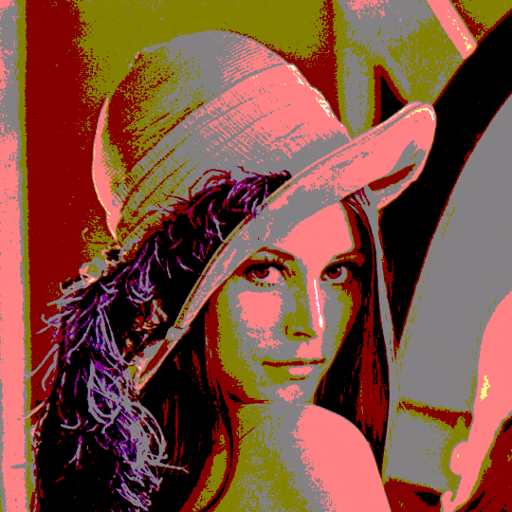
\includegraphics[width=\textwidth]{lena_filter_15}
        \caption{Petnajsti filter}
    \end{subfigure}
    \caption{Primerjava originalne slike z obdelano sliko}
    \label{fig:lena_filter_15}
\end{figure}


\subsubsection*{Filter 16}
\begin{figure}[h]
    \centering
    \begin{subfigure}[b]{0.4\textwidth}
        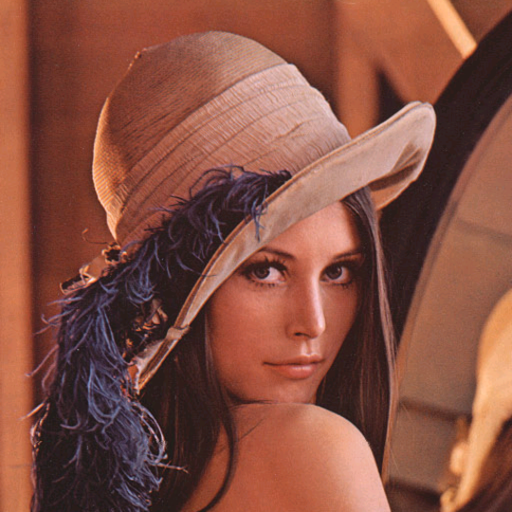
\includegraphics[width=\textwidth]{lena}
        \caption{Original}
    \end{subfigure}
    \begin{subfigure}[b]{0.4\textwidth}
        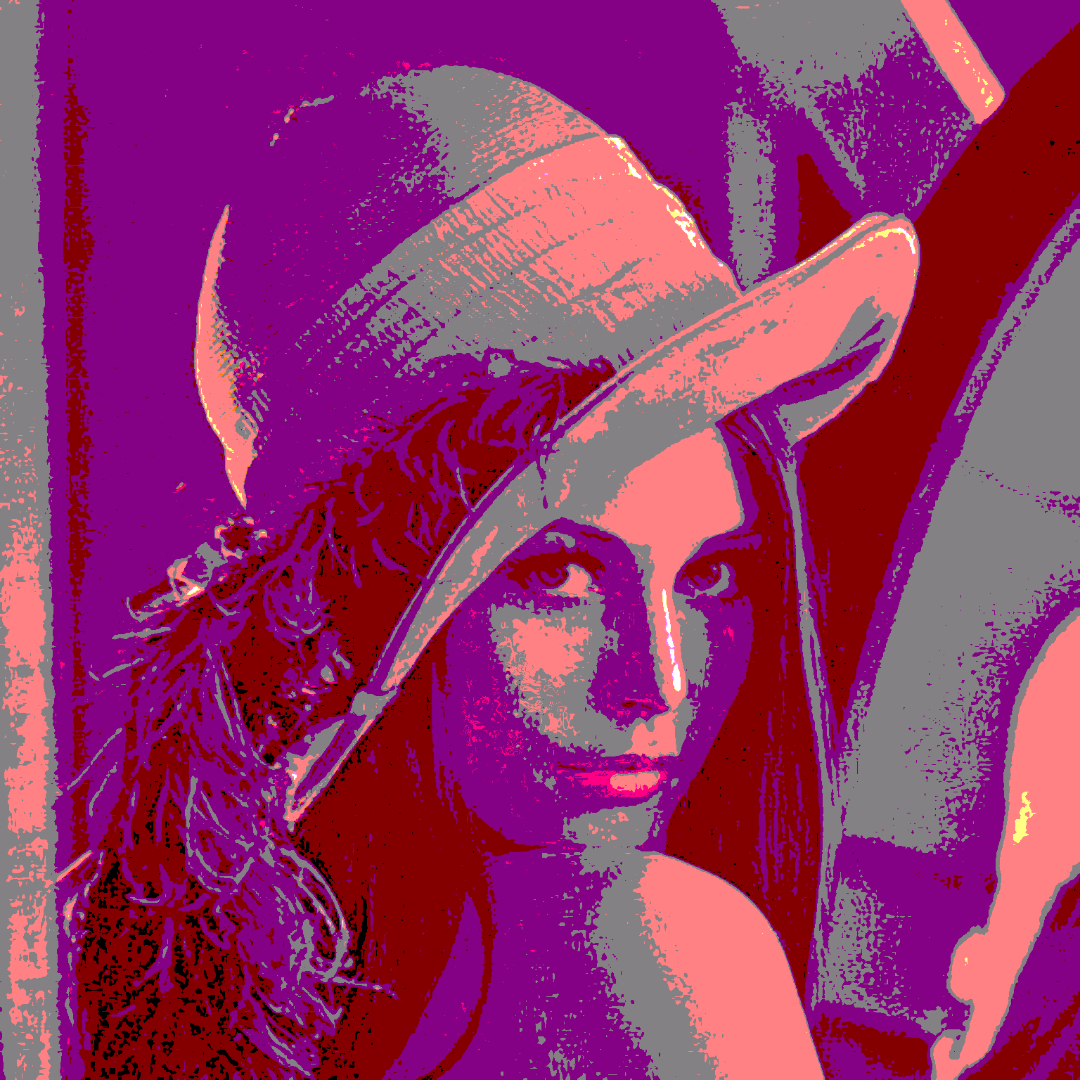
\includegraphics[width=\textwidth]{lena_filter_16}
        \caption{Šestnajsti filter}
    \end{subfigure}
    \caption{Primerjava originalne slike z obdelano sliko}
    \label{fig:lena_filter_16}
\end{figure}


\subsubsection*{Filter 17}
\begin{figure}[h]
    \centering
    \begin{subfigure}[b]{0.4\textwidth}
        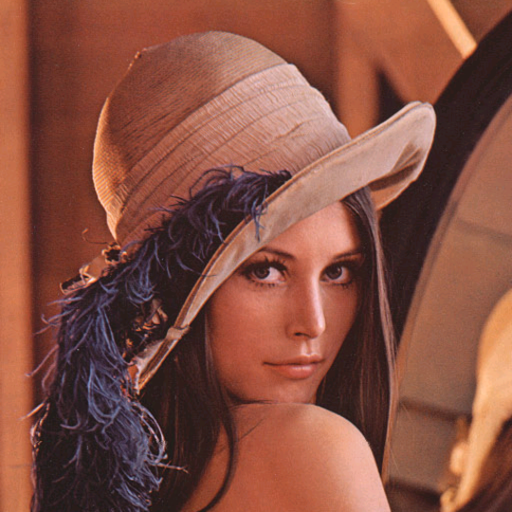
\includegraphics[width=\textwidth]{lena}
        \caption{Original}
    \end{subfigure}
    \begin{subfigure}[b]{0.4\textwidth}
        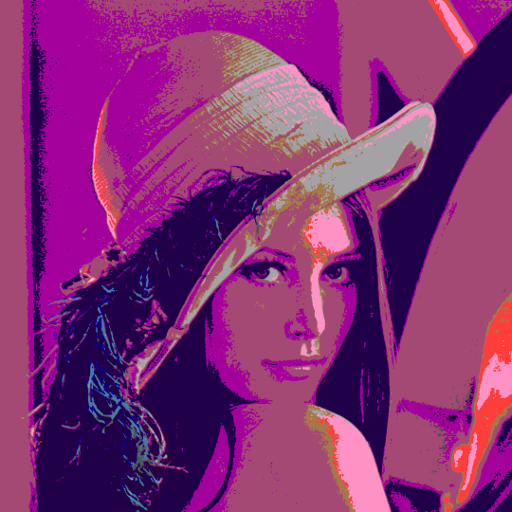
\includegraphics[width=\textwidth]{lena_filter_17}
        \caption{Sedemnajsti filter}
    \end{subfigure}
    \caption{Primerjava originalne slike z obdelano sliko}
    \label{fig:lena_filter_17}
\end{figure}

\chapter{TODO}
Datoteka {\tt magistrska\_naloga.tex} na kratko opisuje, kako se pisanja
magistrskega dela lotimo z uporabo programskega pateka \LaTeX. V tem dokumentu
bomo predstavili nekaj njegovih prednosti in hib. Kar se slednjih tiče, mi
pride na misel ena sama. Ko se srečamo z njim, nam izgleda kot kislo jabolko,
nismo prepričani, da bi želeli vanj ugrizniti. Lahko pa z njim pripravimo
odličen zavitek ali pa pridemo na okus.

Česa od tega dokumenta ne pričakujte? Izkušeni uporabniki \LaTeX{}a bi vse
skupaj zastavili drugače. Morda bi napisali posebno razredno datoteko
(\emph{class file}) --- v resnici priredili katero od obstoječih ---, v
datoteki {\tt magistrska\_naloga.tex} ohranili samo najbolj grobo strukturo in
vanjo vključevali  posamezna po\-glav\-ja. Hkrati s pisanjem teksta bi
poskrbeli tudi za stvarno kazalo ({\tt makeindex}), literaturo pa bi citirali
z uporabo {\BibTeX}{a}. Tega, skratka, v tem dokumentu ne boste našli.

Kaj vseeno najdemo. V Poglavju~\ref{ch1} bomo na hitro spoznali besedilne
konstrukte kot so izreki, enačbe in dokazi. Naučili se bomo, kako se na njih
sklicujemo. Poglavje~\ref{ch2} bo predstavilo vključevanje plovk: slik in
tabel. V Poglavju~\ref{ch3} se bomo srečali s sklicevanjem na literaturo.
Sledil bo samo še zaključek.

\chapter{Sklicevanje na besedilne konstrukte}
\label{ch1}
Matematična ali popolna indukcija je eno prvih orodij, ki jih spoznamo za dokazovanje trditev pri matematičnih predmetih.
\begin{izrek}
\label{iz:1}
Za vsako naravno število $n$ velja
\begin{equation}
n < 2^n.
\label{eq:1}
\end{equation}
\end{izrek}
\begin{dokaz}
Dokazovanje z indukcijo zahteva, da neenakost~\eqref{eq:1} najprej preverimo za najmanjše naravno število --- $0$. Res, ker je $0 < 1 = 2^0$, je neenačba~\eqref{eq:1} za $n=0$ izpolnjena.

Sledi indukcijski korak. S predpostavko, da je neenakost~\eqref{eq:1} veljavna pri nekem naravnem številu $n$, je potrebno pokazati, da je ista neenakost v veljavi tudi pri njegovem nasledniku --- naravnem številu $n+1$. Računajmo.
\begin{align}
n+1 &< 2^n + 1  \label{eq:2}\\
    &\le 2^n + 2^n \label{eq:3}\\
    &= 2^{n+1} \nonumber
\end{align}
Neenakost~\eqref{eq:2} je posledica indukcijske predpostavke, neenakost~\eqref{eq:3} pa enostavno dejstvo, da je za vsako naravno število $n$ izraz $2^n$ vsaj tako velik kot 1. S tem je dokaz Izreka~\ref{iz:1} zaključen.
\end{dokaz}

Opazimo, da je \LaTeX\ številko izreka podredil številki poglavja.


\chapter{Plovke: slike in tabele}
\label{ch2}
Slike in daljše tabele praviloma vključujemo v dokument kot plovke. Pozicija plovke v končnem izdelku ni pogojena s tekom besedila, temveč z izgledom strani. \LaTeX\ bo skušal plovko postaviti samostojno, praviloma na vrh strani, na kateri se na takšno plovko prvič sklicujemo. Pri tem pa bo na vsako stran končnega izdelka želel postaviti tudi sorazmerno velik del besedila. V skrajnem primeru, če imamo res preveč plovk, se bo odločil za stran popolnoma zapolnjeno s plovkami.

\section{Formati slik}
Bitne slike, vektorske slike, kakršnekoli slike, z \LaTeX{}om lahko vključimo vse.
Slika~\ref{pic1} je v {\tt .pdf} formatu.
\begin{figure}
    \begin{center}
        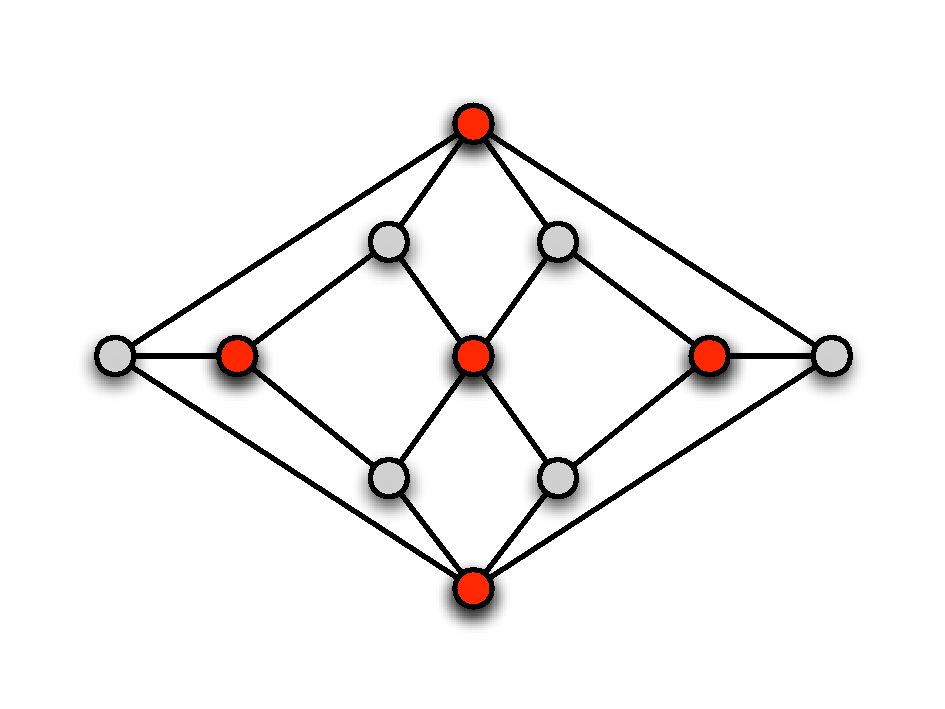
\includegraphics[width=10cm]{pic1.pdf}
    \end{center}
\caption{Herschelov graf, vektorska grafika.}
\label{pic1}
\end{figure}
Pa res lahko vključimo slike katerihkoli formatov? Žal ne. Programski paket \LaTeX\ lahko uporabljamo v več dialektih. Ukaz {\tt latex} ne mara vključenih slik v formatu Portable Document Format {\tt .pdf}, ukaz {\tt pdflatex} pa ne prebavi slik v Encapsulated Postscript Formatu {\tt .eps}.
Strnjeno v Tabeli~\ref{tbl:1}.

\begin{table}
    \begin{center}
        \begin{tabular}{l|ccc}
            ukaz/format & {\tt .pdf} & {\tt .eps} & ostali formati \\ \hline
                        {\tt pdflatex} & da & ne & da \\
                        {\tt latex}   & ne & da  & da
        \end{tabular}
    \end{center}
\caption{}
\label{tbl:1}
\end{table}

Nasvet? Odločite se za uporabo ukaza {\tt pdflatex}. Vaš izdelek bo brez vmesnih stopenj na voljo v {.pdf} formatu in ga lahko odnesete v vsako tiskarno. Če morate na vsak način vključiti sliko, ki jo imate v {\tt .eps} formatu, jo vnaprej pretvorite v alternativni format, denimo {\tt .pdf}.

Včasih se da v okolju za uporabo programskega paketa \LaTeX\ nastaviti na kakšen način bomo prebavljali vhodne dokumente. Spustni meni na Sliki~\ref{pic2} odkriva uporabo \LaTeX{}a v njegovi pdf inkarnaciji --- {\tt pdflatex}.
\begin{figure}
\begin{center}

\includegraphics[width=10cm]{pic2.png}
\end{center}
\caption{Kateri dialekt uporabljati?}
\label{pic2}
\end{figure}

Vključena Slika~\ref{pic2} je seveda bitna.

Kaj pa stran iz študentskega referata?\label{pp}
Tudi njo lahko vključimo v dokument. Toda ne kot plovko.


\chapter{Kaj pa literatura?}
\label{ch3}
Kot smo omenili že v uvodu, je pravi način za citiranje literature uporaba \BibTeX{}a~\cite{bib}.
Programski paket \LaTeX je prvotno predstavljen v priročniku~\cite{lat} in je v resnici nadgradnja sistema \TeX\ avtorja Donalda Knutha, znanega po denimo, če izpustim njegovo umetnost programiranja, Knuth-Bendixovem algoritmu~\cite{dk1}.

Vsem raziskovalcem s področja računalništva pa svetujem v branje mnenje L.\ Fortnowa~\cite{lf}~\cite{trifonova}.

\chapter{Sklepne ugotovitve}
Izbira \LaTeX\ ali ne \LaTeX\ je seveda prepuščena vam samim. Res je, da so prvi koraki v \LaTeX{}u težavni. Ta dokument naj vam služi kot začetna opora pri hoji.
